\chapter{Subdivergences and Forest Formulas}
\label{ch:volume-ii-subdivergences-forest-formulas}

\section{Graphs and Ultraviolet Subgraphs}

Work in a massive Euclidean scalar theory in \(D\) dimensions.  A connected
Feynman graph \(\Gamma\) has a finite set \(E(\Gamma)\) of internal lines, a
finite set \(V(\Gamma)\) of vertices, and external momenta
\[
  p=(p_1,\ldots,p_N),
  \qquad
  \sum_{a=1}^N p_a=0 .
\]
Choose independent loop momenta
\(\ell=(\ell_1,\ldots,\ell_{L(\Gamma)})\), where
\[
  L(\Gamma)=|E(\Gamma)|-|V(\Gamma)|+1 .
\]
With polynomial numerator \(N_\Gamma(\ell,p)\) and propagator masses
\(m_e>0\), the Euclidean momentum-space integrand has the form
\[
  I_\Gamma(\ell,p)
  =
  \frac{N_\Gamma(\ell,p)}
       {\prod_{e\in E(\Gamma)}
        \big(q_e(\ell,p)^2+m_e^2\big)} .
\]
Here \(q_e(\ell,p)\) is the momentum carried by the line \(e\), determined by
the chosen momentum routing.

A subgraph \(\gamma\subseteq\Gamma\) is specified by a subset
\(E(\gamma)\subseteq E(\Gamma)\) together with all vertices incident to those
lines.  The loop number of \(\gamma\) is
\[
  L(\gamma)=|E(\gamma)|-|V(\gamma)|+c(\gamma),
\]
where \(c(\gamma)\) is the number of connected components of \(\gamma\).
The external momenta \(p_\gamma\) of \(\gamma\) consist of the original external
momenta entering \(\gamma\) together with the momenta carried by internal lines
of \(\Gamma\) that meet \(\gamma\) and then leave it.  The contracted graph
\(\Gamma/\gamma\) is obtained by replacing every connected component of
\(\gamma\) by a single vertex.

The ultraviolet scaling associated with \(\gamma\) scales the loop momenta
internal to \(\gamma\) by a common parameter \(\rho\) and keeps \(p_\gamma\)
fixed.  If the leading homogeneous scaling of \(I_\gamma\) is
\[
  \dd^{DL(\gamma)}\ell_\gamma\,
  I_\gamma(\rho\ell_\gamma,p_\gamma)
  =
  O(\rho^{\omega(\gamma)})
  \dd^{DL(\gamma)}\ell_\gamma
  \qquad
  (\rho\to\infty),
\]
then \(\omega(\gamma)\) is the superficial degree of divergence.  For a scalar
graph with numerator degree \(r(\gamma)\),
\[
  \omega(\gamma)
  =
  D L(\gamma)+r(\gamma)-2|E(\gamma)|.
\]
A proper connected one-particle-irreducible subgraph with
\(\omega(\gamma)\ge0\) is called a divergent subgraph.  The word proper means
\(\gamma\ne\Gamma\).  A disconnected subgraph is divergent when each of its
connected components is divergent.

\section{Taylor Operators and Local Vertices}

Fix for each divergent subgraph \(\gamma\) a subtraction point
\(p_\gamma^\ast\) in the space of independent external momenta of \(\gamma\).
The point is chosen away from infrared singularities; for massive Euclidean
graphs, zero momentum is allowed when the relevant Green function is infrared
regular.  Let \(a=(a_1,\ldots,a_M)\) be independent coordinates for
\(p_\gamma-p_\gamma^\ast\).  The Taylor operator of degree \(\omega(\gamma)\)
is
\[
  (t_\gamma f)(p_\gamma)
  =
  \sum_{|\alpha|\le\omega(\gamma)}
  \frac{a^\alpha}{\alpha!}
  \left.
    \partial_a^\alpha f(p_\gamma^\ast+a)
  \right|_{a=0}.
\]
It acts on the dependence of the integrand on the external momenta of
\(\gamma\), while all loop momenta internal to \(\gamma\) remain integration
variables.

The image \(t_\gamma I_\Gamma\) is polynomial in \(p_\gamma\) of degree at most
\(\omega(\gamma)\).  In position space, a polynomial in the momentum entering a
contracted vertex is a finite linear combination of derivatives acting at that
vertex.  Therefore \(t_\gamma I_\Gamma\) represents a local insertion in
\(\Gamma/\gamma\).  This is the graph-level form of the locality statement
established in the preceding chapter.

\begin{figure}[H]
  \centering
  \resizebox{0.96\textwidth}{!}{%
  \begin{tikzpicture}[>=Stealth,x=1cm,y=1cm,every node/.style={font=\small}]
    \tikzset{
      line/.style={line width=0.95pt},
      arr/.style={-{Latex[length=2mm]},line width=0.9pt},
      blob/.style={ellipse,draw=black,fill=gray!15,line width=0.9pt,
        minimum width=1.35cm,minimum height=0.72cm}
    }
    \begin{scope}
      \node[font=\normalsize] at (0,2.0) {subgraph};
      \draw[line] (-2.45,0.55)--(-1.2,0.55);
      \node[blob] (G) at (0,0.55) {\(\gamma\)};
      \draw[line] (G.east)--(2.45,0.55);
      \draw[line] (-0.35,0.05)--(-0.85,-0.95);
      \draw[line] (0.35,0.05)--(0.85,-0.95);
      \node[blue!70!black,align=center] at (0,-1.55)
        {external variables \(p_\gamma\)};
    \end{scope}

    \draw[arr] (3.0,0.55)--(4.35,0.55);
    \node[above] at (3.68,0.72) {\(t_\gamma\)};

    \begin{scope}[shift={(6.3,0)}]
      \node[font=\normalsize] at (0,2.0) {local vertex};
      \draw[line] (-2.45,0.55)--(-0.22,0.55);
      \draw[line] (0.22,0.55)--(2.45,0.55);
      \fill[red!75!black] (0,0.55) circle (3pt);
      \draw[line] (-0.05,0.2)--(-0.75,-0.95);
      \draw[line] (0.05,0.2)--(0.75,-0.95);
      \node[red!75!black,align=center] at (0,-1.55)
        {polynomial in \(p_\gamma\)\\degree \(\le\omega(\gamma)\)};
    \end{scope}

    \draw[arr] (9.15,0.55)--(10.5,0.55);

    \begin{scope}[shift={(12.7,0)}]
      \node[font=\normalsize] at (0,2.0) {contracted graph};
      \draw[line] (-2.1,0.55)--(-0.3,0.55);
      \draw[line] (0.3,0.55)--(2.1,0.55);
      \draw[line] (-0.2,0.18)--(-1.05,-0.95);
      \draw[line] (0.2,0.18)--(1.05,-0.95);
      \node[circle,draw=black,fill=red!15,line width=0.9pt,
        minimum size=0.55cm] at (0,0.55) {\(C_\gamma\)};
      \node[green!45!black,align=center] at (0,-1.55)
        {counterterm insertion\\in \(\Gamma/\gamma\)};
    \end{scope}
  \end{tikzpicture}
  }
  \caption{The Taylor operator \(t_\gamma\) extracts the polynomial part of a
  divergent subgraph in its external variables.  The polynomial is represented
  in the contracted graph by a local counterterm vertex.}
  \label{fig:volume-ii-taylor-subgraph-local-vertex}
\end{figure}

\section{Spinneys, Forests, and the Recursive R-Operation}

A spinney \(S\) of \(\Gamma\) is a finite set of mutually disjoint divergent
proper subgraphs of \(\Gamma\).  Mutually disjoint means that no internal line
or vertex is shared.  The empty set is allowed.  A forest \(F\) of \(\Gamma\)
is a finite set of divergent subgraphs such that any two elements of \(F\) are
either disjoint or nested:
\[
  \gamma_1\cap\gamma_2=\emptyset,
  \qquad
  \gamma_1\subset\gamma_2,
  \qquad
  \hbox{or}
  \qquad
  \gamma_2\subset\gamma_1 .
\]
The full graph \(\Gamma\) is included among the possible forest elements when
\(\omega(\Gamma)\ge0\).  The empty forest is allowed.

\begin{figure}[H]
  \centering
  \resizebox{0.94\textwidth}{!}{%
  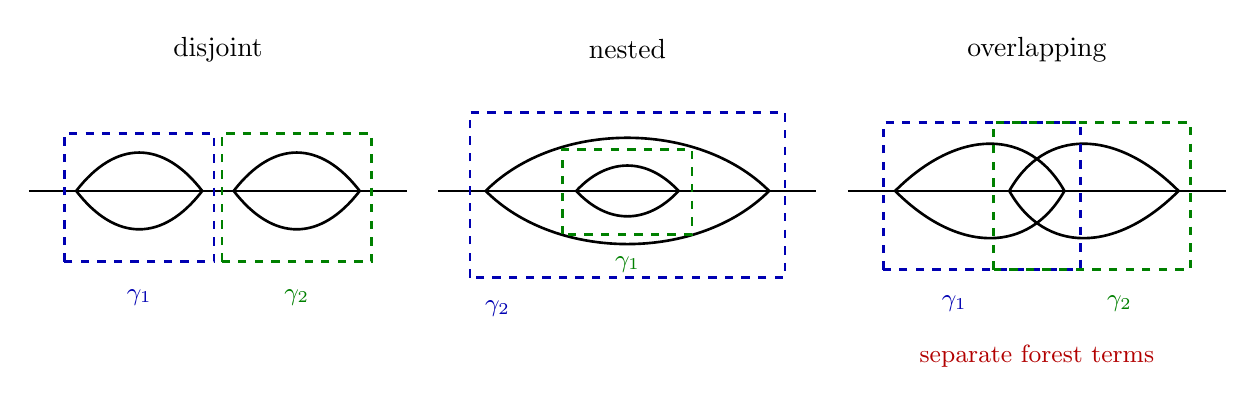
\begin{tikzpicture}[x=1cm,y=1cm,every node/.style={font=\small}]
    \tikzset{line/.style={line width=0.95pt}}
    \begin{scope}
      \node[font=\normalsize] at (0,2.35) {disjoint};
      \draw[line] (-2.4,0.55)--(2.4,0.55);
      \draw[line] (-1.8,0.55)..controls (-1.3,1.2) and (-0.7,1.2)..(-0.2,0.55);
      \draw[line] (-1.8,0.55)..controls (-1.3,-0.1) and (-0.7,-0.1)..(-0.2,0.55);
      \draw[line] (0.2,0.55)..controls (0.7,1.2) and (1.3,1.2)..(1.8,0.55);
      \draw[line] (0.2,0.55)..controls (0.7,-0.1) and (1.3,-0.1)..(1.8,0.55);
      \draw[blue!70!black,dashed,line width=1pt] (-1.95,-0.35) rectangle (-0.05,1.28);
      \draw[green!50!black,dashed,line width=1pt] (0.05,-0.35) rectangle (1.95,1.28);
      \node[blue!70!black] at (-1.0,-0.8) {\(\gamma_1\)};
      \node[green!50!black] at (1.0,-0.8) {\(\gamma_2\)};
    \end{scope}

    \begin{scope}[shift={(5.2,0)}]
      \node[font=\normalsize] at (0,2.35) {nested};
      \draw[line] (-2.4,0.55)--(2.4,0.55);
      \draw[line] (-1.8,0.55)..controls (-0.9,1.45) and (0.9,1.45)..(1.8,0.55);
      \draw[line] (-1.8,0.55)..controls (-0.9,-0.35) and (0.9,-0.35)..(1.8,0.55);
      \draw[line] (-0.65,0.55)..controls (-0.25,0.98) and (0.25,0.98)..(0.65,0.55);
      \draw[line] (-0.65,0.55)..controls (-0.25,0.12) and (0.25,0.12)..(0.65,0.55);
      \draw[blue!70!black,dashed,line width=1pt] (-2.0,-0.55) rectangle (2.0,1.55);
      \draw[green!50!black,dashed,line width=1pt] (-0.82,0.0) rectangle (0.82,1.08);
      \node[blue!70!black] at (-1.65,-0.95) {\(\gamma_2\)};
      \node[green!50!black] at (0,-0.38) {\(\gamma_1\)};
    \end{scope}

    \begin{scope}[shift={(10.4,0)}]
      \node[font=\normalsize] at (0,2.35) {overlapping};
      \draw[line] (-2.4,0.55)--(2.4,0.55);
      \draw[line] (-1.8,0.55)..controls (-1.0,1.35) and (-0.1,1.35)..(0.35,0.55);
      \draw[line] (-1.8,0.55)..controls (-1.0,-0.25) and (-0.1,-0.25)..(0.35,0.55);
      \draw[line] (-0.35,0.55)..controls (0.1,1.35) and (1.0,1.35)..(1.8,0.55);
      \draw[line] (-0.35,0.55)..controls (0.1,-0.25) and (1.0,-0.25)..(1.8,0.55);
      \draw[blue!70!black,dashed,line width=1pt] (-1.95,-0.45) rectangle (0.55,1.42);
      \draw[green!50!black,dashed,line width=1pt] (-0.55,-0.45) rectangle (1.95,1.42);
      \node[blue!70!black] at (-1.05,-0.88) {\(\gamma_1\)};
      \node[green!50!black] at (1.05,-0.88) {\(\gamma_2\)};
      \node[red!70!black,align=center] at (0,-1.55)
        {separate forest terms};
    \end{scope}
  \end{tikzpicture}
  }
  \caption{A forest contains compatible divergent subgraphs: disjoint or
  nested collections are compatible.  Overlapping subgraphs are handled by
  separate forest terms.}
  \label{fig:volume-ii-compatible-forests}
\end{figure}

The recursive construction is most transparent when written in two steps.
First define the prepared integrand
\[
  \overline R_\Gamma I_\Gamma
  =
  I_\Gamma
  +
  \sum_{\substack{S\ {\rm spinney\ of}\ \Gamma\\S\ne\emptyset}}
  \left(\prod_{\gamma\in S} C_\gamma\right) I_\Gamma .
\]
The product of \(C_\gamma\)'s means: replace each disjoint subgraph
\(\gamma\) by its counterterm vertex in the graph \(\Gamma/S\).  Since the
elements of a spinney are disjoint, these replacements can be made
simultaneously.  The counterterm attached to a connected divergent graph is
defined recursively by
\[
  C_\gamma I_\gamma
  =
  -\,t_\gamma\,\overline R_\gamma I_\gamma .
\]
Thus the counterterm of \(\gamma\) is the negative Taylor polynomial of the
subgraph after its own proper subdivergences have already been prepared.

The full \(R\)-operation is
\[
  R_\Gamma I_\Gamma
  =
  \begin{cases}
    (1-t_\Gamma)\,\overline R_\Gamma I_\Gamma,
      & \omega(\Gamma)\ge0,\\[4pt]
    \overline R_\Gamma I_\Gamma,
      & \omega(\Gamma)<0.
  \end{cases}
\]
This formula enforces the order of operations: proper subdivergences are
subtracted inside \(\overline R_\Gamma\), and the overall Taylor subtraction
is applied afterward when the whole graph is superficially divergent.

\section{The Forest Formula}

Let \(\mathfrak F(\Gamma)\) be the set of forests whose elements are divergent
subgraphs of \(\Gamma\), including \(\Gamma\) itself when \(\omega(\Gamma)\ge0\).
For \(F\in\mathfrak F(\Gamma)\), define \(t_F\) by applying \(t_\gamma\) from
smaller subgraphs to larger subgraphs.  If two elements are disjoint, their
operators commute.  The forest formula is
\[
  R_\Gamma I_\Gamma
  =
  \sum_{F\in\mathfrak F(\Gamma)}
  (-1)^{|F|}\,t_F I_\Gamma ,
\]
with \(t_\emptyset=1\).  This compact formula is equivalent to the recursive
definition above: expanding the recursion gives one term for every compatible
choice of subtractions, and the sign records how many Taylor extractions have
been made.

The inclusion-exclusion structure can be seen directly in a graph with one
proper divergent subgraph \(\gamma\) and a divergent overall graph \(\Gamma\).
The possible forests are
\[
  \emptyset,\qquad
  \{\gamma\},\qquad
  \{\Gamma\},\qquad
  \{\gamma,\Gamma\}.
\]
The corresponding operator is
\[
  R_\Gamma
  =
  1-t_\gamma-t_\Gamma+t_\Gamma t_\gamma
  =
  (1-t_\Gamma)(1-t_\gamma),
\]
where \(t_\gamma\) acts before \(t_\Gamma\).  The last term restores the part
subtracted twice at the boundary where the subgraph and the whole graph shrink
in a nested way.

\section{Order of Subtractions and Scale Hierarchies}

The prescription that \(t_\gamma\) acts before \(t_\Gamma\) for
\(\gamma\subset\Gamma\) is forced by the geometry of ultraviolet limits.  A
nested forest represents a hierarchy of large internal momenta.  For example,
if loop momenta internal to \(\gamma\) are of size \(\rho\sigma\) and the
remaining loop momenta of \(\Gamma/\gamma\) are of size \(\rho\), with
\(\sigma\to\infty\) before \(\rho\to\infty\), then the innermost singular
region is the subgraph \(\gamma\).  Its Taylor polynomial must first be
converted into a local vertex of the contracted graph.  Only after that
replacement is made does the overall Taylor operator see the correct local
integrand for the larger graph.

This ordering can be expressed algebraically.  If
\[
  C_\gamma I_\gamma=-t_\gamma\overline R_\gamma I_\gamma,
\]
then the term \(t_\Gamma t_\gamma I_\Gamma\) in a forest is interpreted as
\[
  t_\Gamma\bigl((t_\gamma I_\gamma)\,I_{\Gamma/\gamma}\bigr),
\]
where \(t_\gamma I_\gamma\) is a polynomial in the external momenta entering
\(\gamma\).  The polynomial is part of the local vertex data of
\(\Gamma/\gamma\), so the overall subtraction is again a Taylor polynomial in
the external momenta of \(\Gamma\).  This is the mechanism by which nested
subtractions preserve locality.

Overlapping divergent subgraphs do not define a single common hierarchy in
which both are innermost subgraphs.  They are therefore not placed in the same
forest.  Their overlap is covered by the sum over compatible forests together
with the overall subtraction.  The apparent combinatorics is the bookkeeping
required for a single local expression to subtract all ultraviolet boundary
regions without assigning a nonlocal counterterm to an overlap.

\section{The Two-Loop Self-Energy Forest}

Return to the two-loop self-energy graph in the six-dimensional cubic theory.
Let \(\Gamma\) be the full graph and let \(\gamma_L,\gamma_R\) denote the left
and right one-loop self-energy subgraphs.  These two subgraphs overlap: they
share the central propagator.  Therefore the forest set is
\[
  \emptyset,\quad
  \{\gamma_L\},\quad
  \{\gamma_R\},\quad
  \{\Gamma\},\quad
  \{\gamma_L,\Gamma\},\quad
  \{\gamma_R,\Gamma\}.
\]
The overlap of \(\gamma_L\) and \(\gamma_R\) is represented by the two separate
one-subgraph forests \(\{\gamma_L\}\) and \(\{\gamma_R\}\), together with their
nested overall forests.

For this graph the \(R\)-operation is
\[
\begin{aligned}
  R_\Gamma I_\Gamma
  &=
  I_\Gamma
  -t_{\gamma_L}I_\Gamma
  -t_{\gamma_R}I_\Gamma
  -t_\Gamma I_\Gamma        \\
  &\quad
  +t_\Gamma t_{\gamma_L}I_\Gamma
  +t_\Gamma t_{\gamma_R}I_\Gamma .
\end{aligned}
\]
The first two subgraph subtraction terms remove the two Schwinger-parameter
boundary regions
\[
  \alpha_1,\alpha_2,\alpha_5\to0,
  \qquad
  \alpha_3,\alpha_4,\alpha_5\to0 .
\]
After these subtractions, the remaining overall boundary
\(\alpha_1,\ldots,\alpha_5\to0\) is subtracted by \(t_\Gamma\).  Since
\(\omega(\Gamma)=2\) for the self-energy in \(D=6\), \(t_\Gamma\) extracts the
constant and quadratic terms in the external momentum.  The final counterterm
is therefore a linear combination of the local operators \(\phi^2\) and
\(\partial_\mu\phi\,\partial_\mu\phi\).

\begin{figure}[H]
  \centering
  \resizebox{0.97\textwidth}{!}{%
  \begin{tikzpicture}[>=Stealth,x=1cm,y=1cm,every node/.style={font=\small}]
    \tikzset{line/.style={line width=0.95pt}}
    \begin{scope}
      \node[font=\normalsize] at (0,2.5) {overlapping subdivergences};
      \draw[line] (-3.0,0.65)--(-2.1,0.65);
      \draw[line] (-2.1,0.65)..controls (-1.35,1.55) and (-0.45,1.55)..(0.0,0.65);
      \draw[line] (-2.1,0.65)..controls (-1.35,-0.25) and (-0.45,-0.25)..(0.0,0.65);
      \draw[line] (0.0,0.65)..controls (0.45,1.55) and (1.35,1.55)..(2.1,0.65);
      \draw[line] (0.0,0.65)..controls (0.45,-0.25) and (1.35,-0.25)..(2.1,0.65);
      \draw[line] (2.1,0.65)--(3.0,0.65);
      \draw[blue!70!black,dashed,line width=1pt] (-2.32,-0.47) rectangle (0.28,1.72);
      \draw[green!50!black,dashed,line width=1pt] (-0.28,-0.47) rectangle (2.32,1.72);
      \draw[red!70!black,dotted,line width=1.2pt] (-2.62,-0.78) rectangle (2.62,2.0);
      \node[blue!70!black] at (-1.15,-0.9) {\(\gamma_L\)};
      \node[green!50!black] at (1.15,-0.9) {\(\gamma_R\)};
      \node[red!70!black] at (0,2.18) {\(\Gamma\)};
    \end{scope}

    \begin{scope}[shift={(7.5,0)}]
      \node[font=\normalsize] at (0,2.5) {forest terms};
      \node[align=left,anchor=west] at (-2.6,1.45)
        {\(\emptyset\)};
      \node[align=left,anchor=west] at (-2.6,0.95)
        {\(\{\gamma_L\},\ \{\gamma_R\}\)};
      \node[align=left,anchor=west] at (-2.6,0.45)
        {\(\{\Gamma\}\)};
      \node[align=left,anchor=west] at (-2.6,-0.05)
        {\(\{\gamma_L,\Gamma\},\ \{\gamma_R,\Gamma\}\)};
      \draw[red!70!black,line width=0.9pt] (-2.55,-0.58)--(2.35,-0.58);
      \node[red!70!black,align=center] at (0,-1.08)
        {overlap represented separately};
    \end{scope}
  \end{tikzpicture}
  }
  \caption{The two one-loop subdivergences of the diamond graph overlap along
  one internal line.  The forest formula treats them in separate compatible
  forests, while the overall graph is subtracted after either one-loop
  subgraph subtraction.}
  \label{fig:volume-ii-diamond-forest-formula}
\end{figure}

\section{Finiteness and Locality}

\begin{theorem}[BPHZ finiteness for massive Euclidean scalar graphs]
Let \(\Gamma\) be a connected Euclidean Feynman graph in a massive scalar
theory.  Assume that all external momenta and subtraction points are chosen
away from infrared singularities, and that \(t_\gamma\) subtracts every
divergent 1PI subgraph \(\gamma\) through degree \(\omega(\gamma)\).  Then
\[
  \int \prod_{i=1}^{L(\Gamma)}\dd^D\ell_i\,
  R_\Gamma I_\Gamma(\ell,p)
\]
is ultraviolet finite.  The counterterm produced by each connected divergent
subgraph is a polynomial in \(p_\gamma\) of degree at most \(\omega(\gamma)\).
\end{theorem}

The proof is a scaling argument organized by the forest decomposition of
ultraviolet regions.  In each sector of large loop momenta, the set of
subgraphs whose internal momenta become large in a common scale hierarchy is a
forest.  For the innermost element \(\gamma\) in that forest, Taylor's theorem
gives
\[
  f(p_\gamma)
  -
  t_\gamma f(p_\gamma)
  =
  \sum_{|\alpha|=\omega(\gamma)+1}
  a^\alpha
  \int_0^1
  \frac{(1-s)^{\omega(\gamma)}}{\omega(\gamma)!}
  \left(\partial_a^\alpha f\right)(p_\gamma^\ast+s a)\,\dd s .
\]
The extra power of \(a\) improves the ultraviolet scaling by one order beyond
the superficial degree assigned to \(\gamma\).  Applying the same argument
from the innermost subgraphs outward improves every boundary region in the
sector.  The inclusion-exclusion signs in the forest formula assemble these
sector subtractions into a single expression independent of the sector
decomposition.  Since all masses are positive and the subtraction points avoid
infrared singularities, the remaining possible divergences are exactly these
ultraviolet boundary regions, and the renormalized integral is finite.

The locality statement follows before integration: every \(C_\gamma\) is a
Taylor polynomial in \(p_\gamma\).  In a theory whose power-counting
counterterms belong to a finite local operator space, the recursive operation
therefore remains inside that same finite space.  This proves perturbative
renormalizability in the finite-list sense used in the previous chapter.

\section{Finite Parts and Subtraction Coordinates}

The Taylor operator includes a choice of subtraction point and a choice of
finite polynomial part.  Changing these choices replaces \(C_\gamma\) by
\[
  C_\gamma+\Delta C_\gamma,
\]
where \(\Delta C_\gamma\) is again a local polynomial in \(p_\gamma\) of degree
at most \(\omega(\gamma)\).  Hence a change of subtraction prescription is a
local redefinition of the parameters multiplying local operators.  The
renormalized amplitudes expressed in one set of physical coordinates can be
re-expressed in another by a finite local change of coordinates.

The next chapter uses this freedom actively.  A family of subtraction
conditions indexed by a Euclidean momentum scale \(\mu\) gives
scale-dependent renormalized couplings.  The differential comparison of
neighboring values of \(\mu\) is the 1PI renormalization group.
